\usepackage{ucll-code}
\usepackage{siunitx}
\usepackage{ifthen}

\usetikzlibrary{positioning}

\makeatletter
\def\light@caption@on{on}
\def\light@caption@off{off}
\def\light@caption@neutral{}
\makeatother

\newcommand{\hex}[1]{\texttt{\bfseries #1}}


\title{Data Compression: LZ77}
\author{Fr\'ed\'eric Vogels}

\begin{document}

\begin{frame}
  \titlepage
\end{frame}

\begin{frame}
  \frametitle{Disclaimer}
  \begin{center}
    \Large
    Most examples assume we deal with text,
    but the principles apply to bytes in general
  \end{center}
\end{frame}

\begin{frame}
  \frametitle{Compression Algorithms}
  \begin{itemize}
    \item GQU
          \begin{itemize}
            \item Example algorithm
            \item Assumes pairs of bytes occur often
          \end{itemize}
    \item RLE
          \begin{itemize}
            \item Assumes long runs of the same value occur often
            \item TGA, PCX, fax machines
          \end{itemize}
    \item Huffman
          \begin{itemize}
            \item Assumes certain bytes occur more often
            \item Widely used (MP3, JPEG, zip, web, \dots)
          \end{itemize}
    \item<2-> LZ77/LZ78/LZSS/LZMA/\dots
          \begin{itemize}
            \item Assumes same series of bytes occur repeatedly
            \item Widely used (zip, 7z, rar, png, \dots)
          \end{itemize}
  \end{itemize}
\end{frame}

{
  \newcommand{\drawbox}[1]{\draw (#1.south west) rectangle (#1.north east);}
  \begin{frame}
    \frametitle{Example Input}
    \code[language={},font=\small,width=\linewidth,frame=none]{singer.txt}
    \begin{tikzpicture}[overlay,remember picture,ref/.style={-latex,thick}]
      \visible<2->{
        \drawbox{inger1}
        \drawbox{inger2}
        \draw[ref] (inger2.east) to[bend right=30] (inger1.east);
      }

      \visible<3->{
        \drawbox{hoort1}
        \drawbox{hoort2}
        \draw[ref] (hoort2.east) to[bend right=30] (hoort1.east);
      }

      \visible<4->{
        \draw (singer1.north west) rectangle (inger2.south east);
        \drawbox{singer2}
        \draw[ref] (singer2.north) to[bend right=30] (inger2.east);
      }

      \visible<5->{
        \drawbox{naaimasjien1}
        \drawbox{naaimasjien2}
        \draw[ref] (naaimasjien2.north) to[bend right=30] (naaimasjien1.east);
      }

      \visible<6->{
        \drawbox{wat1}
        \drawbox{wat2}
        \draw[ref] (wat2.east) to[bend right=30] (wat1.east);
      }

      \visible<7->{
        \drawbox{jespers1}
        \drawbox{jespers2}
        \draw[ref] (jespers2.east) to[bend right=30] (jespers1.south);
      }

      \visible<8->{
        \drawbox{singer3}
        \drawbox{singer2}
        \draw[ref] (singer3.north east) to[bend right=10] (singer2.south);
      }

      \visible<9->{
        \drawbox{naaimasjien3}
        \drawbox{naaimasjien2}
        \draw[ref] (naaimasjien3.north east) to[bend right=10] (naaimasjien2.south);
      }
    \end{tikzpicture}
  \end{frame}
}

\begin{frame}
  \frametitle{Observations}
  \begin{itemize}
    \item Same words are repeated often
    \item Happens often in certain data files
          \begin{itemize}
            \item Source code (keywords, identifiers, etc.)
            \item Text files (word, pdf, etc.)
            \item XML
            \item \dots
          \end{itemize}
    \item More generally: certain series of bytes occur repeatedly
    \item We can use this to our advantage
  \end{itemize}
\end{frame}

\begin{frame}
  \frametitle{Basic Principle of LZ77}
  \begin{itemize}
    \item If same word has appeared before\dots
    \item \dots don't repeat it
    \item \dots but refer to the previous occurence
  \end{itemize}
\end{frame}

{
  \newcommand{\chunk}[3]{
    \draw[|-|] ($ (#1.south west) + (0,-0.1) $) -- ($ (#1.south east) + (0,-0.1) $);
    \draw[|->] ($ (#2.south west) + (0,-0.1) $) -- ($ (#2.south east) + (0,-0.1) $) node[midway,below,font=\tiny] {#3};
    \draw[-latex] ($ (#1.south) + (0,-0.1) $) -- ++(0,-0.5) -| ($ (#2.south west) + (0,-0.2) $);
  }
  \newcommand{\multichunk}[5]{
    \draw[|-|] ($ (#1.south west) + (0,-0.1) $) -- ($ (#2.south east) + (0,-0.1) $);
    \draw[|->] ($ (#3.south west) + (0,-0.1) $) -- ($ (#4.south east) + (0,-0.1) $) node[midway,below,font=\tiny] {#5};
    \draw[-latex] ($ (#1.south) ! 0.5 ! (#2.south) + (0,-0.1) $) -- ++(0,-0.5) -| ($ (#3.south west) + (0,-0.2) $);
  }
  \begin{frame}
    \frametitle{Conceptual Example}
    \structure{Data to be compressed}
    \begin{center} \tt
      \NODE{\alert<2>{mux}}{mux1}\NODE{\alert<3>{mux}}{mux2}\NODE{\alert<4>{bar}}{bar1}\NODE{\alert<5>{bar}}{bar2}\NODE{\alert<6>{muxbarbar}}{muxbarbar}\NODE{\alert<7>{muxmuxbarbarmuxbarbar}}{last}
    \end{center}
    \begin{tikzpicture}[overlay,remember picture]
      \visible<handout:0|3>{
        \chunk{mux2}{mux1}{3}
      }

      \visible<handout:0|5>{
        \chunk{bar2}{bar1}{3}
      }

      \visible<handout:0|6>{
        \multichunk{muxbarbar}{muxbarbar}{mux2}{bar2}{6}
      }

      \visible<handout:0|7>{
        \multichunk{last}{last}{mux1}{muxbarbar}{21}
      }
    \end{tikzpicture}
    \vskip5mm
    \structure{Compressed form}
    \begin{enumerate}
      \item<2-> {\tt mux}
      \item<3-> Repeat 3 letters starting from first letter
      \item<4-> {\tt bar}
      \item<5-> Repeat 3 letters starting from 6th letter
      \item<6-> Repeat 6 letters starting from 3rd letter
      \item<7-> Repeat 21 letters starting from first letter
    \end{enumerate}
  \end{frame}
}

\begin{frame}
  \frametitle{Resolving Technical Difficulties}
  \begin{itemize}
    \item Conceptually, LZ works by referring to past data
    \item We still need to find a way to encode this into bytes
    \item We need to make sure a decompressor can unambiguously reconstruct the original data
  \end{itemize}
\end{frame}

\begin{frame}
  \frametitle{First Attempt}
  \begin{itemize}
    \item A back reference consists of two components
          \begin{itemize}
            \item Start location of data to be repeated
            \item How many bytes to repeat
          \end{itemize}
    \item Let's use a single byte for each
  \end{itemize}

  \begin{center}
    \begin{tabular}{l@{$\;\rightarrow\;$}l}
      {\tt mux} & \tt \hex{6D} \hex{75} \hex{78} \\
      Repeat 3 letters starting from first letter & \tt \hex{00} \hex{03} \\
      {\tt bar} & \tt \hex{62} \hex{61} \hex{72} \\
      Repeat 3 letters starting from 6th letter & \tt \hex{05} \hex{03} \\
      Repeat 6 letters starting from 3rd letter & \tt \hex{02} \hex{06} \\
      Repeat 21 letters starting from first letter & \tt \hex{00} \hex{15} \\
    \end{tabular}
  \end{center}
\end{frame}

\begin{frame}
  \frametitle{Ambiguity Problem}
  \begin{center}
    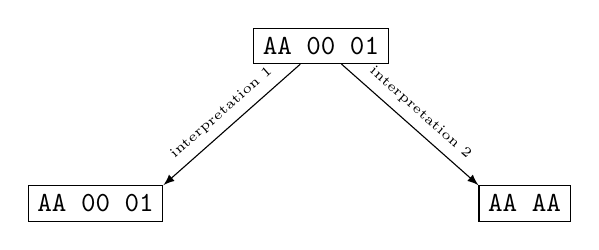
\begin{tikzpicture}
      \node[font=\tt,draw] (original) at (0,0) {\hex{AA} \hex{00} \hex{01}};
      \node[font=\tt,anchor=east,draw] (decompression 1) at (-2,-2) {\hex{AA} \hex{00} \hex{01}};
      \node[font=\tt,anchor=west,draw] (decompression 2) at (2,-2) {\hex{AA} \hex{AA}};

      \draw[-latex] (original) -- (decompression 1.north east) node[midway,above,sloped,font=\tiny] {interpretation 1};
      \draw[-latex] (original) -- (decompression 2.north west) node[midway,above,sloped,font=\tiny] {interpretation 2};
    \end{tikzpicture}
  \end{center}

  \begin{itemize}
    \item How to differentiate between
          \begin{itemize}
            \item A literal byte
            \item A reference to previous data
          \end{itemize}
    \item Interpretation 1: {\tt 00 01} is data
    \item Interpretation 2: {\tt 00 01} is a reference to past data \\ (start at index 0, length 1)
  \end{itemize}
\end{frame}

\begin{frame}
  \frametitle{Solution To Ambiguity Problem}
  \begin{itemize}
    \item Many solutions possible
    \item LZ77 imposes uniformity
    \item LZ77 does not discern between literal bytes and back reference bytes
    \item In LZ77, everything is a back reference
    \item This of course leads to a new problem
  \end{itemize}
\end{frame}

\begin{frame}
  \frametitle{The Case Of The Missing Literal Bytes}
  \structure{Data to be compressed}
  \begin{center}
    \tt muxmuxbarbarmuxbarbarmuxmuxbarbarmuxbarbar
  \end{center}
  \vskip5mm
  \structure{Our ordeal}
  \begin{itemize}
    \item LZ77 allows only back references
    \item How to start compressing above data?
    \item {\tt m} has never been encountered before
    \item So no back reference possible
    \item We're stuck!
  \end{itemize}
\end{frame}

\begin{frame}
  \frametitle{LZ77's Approach}
  \begin{itemize}
    \item LZ77 sees data as series of triplets
    \item<2-> Location of repeated data
              \begin{itemize}
                \item Expressed in ``how many bytes ago''
                \item Why? \cake
              \end{itemize}
    \item<3-> Length of repeated data
    \item<4-> Single extra datum
    \item<4-> If $x$ is new byte $\rightarrow$ (0, 0, $x$)
    \item<4-> Why best use 0,0 and not 5,0? \cake
  \end{itemize}
  \begin{center}
    \begin{tikzpicture}[byte/.style={minimum width=0.75cm,minimum height=1cm,draw}]
      \node[byte] (first) at (0,0) {};
      \node[byte] (second) at (1,0) {};
      \node[byte] (third) at (2,0) {};

      \draw[|-|] ($ (first.south west) + (0,-0.5) $) -- ($ (third.south east) + (0,-0.5) $) node[midway,below,font=\small] {triplet};

      \visible<2->{
        \node[anchor=west] (loc) at (3,2) {Location};
        \draw[-latex] (first.north) |- (loc.west);
      }

      \visible<3->{
        \node[anchor=north west] (len) at (loc.south west) {Length};
        \draw[-latex] (second.north) |- (len.west);
      }

      \visible<4->{
        \node[anchor=north west] (slb) at (len.south west) {Datum};
        \draw[-latex] (third.north) |- (slb.west);
      }
    \end{tikzpicture}
  \end{center}
\end{frame}

\begin{frame}
  \frametitle{Practical Example}
  \structure{Data to be compressed}
  \begin{center}
    \tt\only<handout:0|1->{\alert<1-2>{m}\alert<3-4>{u}\alert<5-6>{x}{\only<7-8>{\color{green}}mux}\alert<7-8>{b}\alert<9-10>{a}\alert<11-12>{r}{\only<13-14>{\color{green}}bar}\alert<13-14>{m}%
    {\only<15-16>{\color{green}}uxbarbarm}\alert<15-16>{u}{\only<17-18>{\color{green}}xmuxbarbarmuxbarbar}\alert<17-18>{b}{\only<19-20>{\color{green}}armu}\alert<19-20>{x}}
    \tt\only<handout:1-|0>{\alert<handout:1>{m}\alert<handout:2>{u}\alert<handout:3>{x}{\only<handout:4>{\color{green}}mux}\alert<handout:4>{b}\alert<handout:5>{a}\alert<handout:6>{r}{\only<handout:7>{\color{green}}bar}\alert<handout:7>{m}%
    {\only<handout:8>{\color{green}}uxbarbarm}\alert<handout:8>{u}{\only<handout:9>{\color{green}}xmuxbarbarmuxbarbar}\alert<handout:9>{b}{\only<handout:10>{\color{green}}armu}\alert<handout:10>{x}}
  \end{center}
  \structure{Explanation}
  \begin{overprint}
    \onslide<handout:1|1-2>
    \begin{itemize}
      \item First datum: {\tt m} (hex \hex{6D})
      \item Has not appeared before
      \item We use 0 as position and length to indicate this
      \item Extra datum: \hex{6D}
    \end{itemize}

    \onslide<handout:2|3-4>
    \begin{itemize}
      \item Second datum: {\tt u} (hex \hex{75})
      \item Has not appeared before
      \item We use 0 as position and length to indicate this
      \item Extra datum: \hex{75}
    \end{itemize}

    \onslide<handout:3|5-6>
    \begin{itemize}
      \item Third datum: {\tt x} (hex \hex{78})
      \item Has not appeared before
      \item We use 0 as position and length to indicate this
      \item Extra datum: \hex{78}
    \end{itemize}

    \onslide<handout:4|7-8>
    \begin{itemize}
      \item {\tt m} encountered before
      \item We take longest possible match
      \item {\tt\color{green} mux} is longest match
      \item Location = 3 bytes ago, length = 3
      \item Obligatory extra datum: {\tt b} (hex \hex{62})
    \end{itemize}

    \onslide<handout:5|9-10>
    \begin{itemize}
      \item {\tt a} is new
      \item Location: 0, length = 0
      \item Extra datum: {\tt a} (hex \hex{61})
    \end{itemize}

    \onslide<handout:6|11-12>
    \begin{itemize}
      \item {\tt r} is new
      \item Location: 0, length = 0
      \item Extra datum: {\tt r} (hex \hex{72})
    \end{itemize}

    \onslide<handout:7|13-14>
    \begin{itemize}
      \item {\tt bar} looks familiar
      \item Location: 3 bytes ago, length = 3
      \item Extra datum: {\tt m} (hex \hex{6D})
    \end{itemize}

    \onslide<handout:8|15-16>
    \begin{itemize}
      \item Longest match: {\tt uxbarbarm}
      \item Location: 9 bytes ago, length = 9
      \item Extra datum: {\tt u} (hex \hex{75})
    \end{itemize}

    \onslide<handout:9|17-18>
    \begin{itemize}
      \item Longest match: {\tt xmuxbarbarmuxbarbar}
      \item Location: 21 bytes ago, length = 19
      \item 21 in hex: \hex{15}, 19 in hex: \hex{13}
      \item Extra datum: {\tt b} (hex \hex{62})
    \end{itemize}

    \onslide<handout:10|19-20>
    \begin{itemize}
      \item Longest match: {\tt armux}
      \item Oops, no extra datum left
      \item Longest match that leaves extra datum: {\tt armu}
      \item Location: 12 bytes ago, length = 4
      \item Extra datum: {\tt x} (hex \hex{78})
    \end{itemize}

  \end{overprint}
  \vskip4mm
  \structure{Compressed form}
  \begin{center} \tt
    \parbox{9cm}{
      \visible<handout:1-|2->{\alert<2>{\hex{00} \hex{00} \hex{6D}}}
      \visible<handout:2-|4->{\alert<4>{\hex{00} \hex{00} \hex{75}}}
      \visible<handout:3-|6->{\alert<6>{\hex{00} \hex{00} \hex{78}}}
      \visible<handout:4-|8->{\alert<8>{\hex{03} \hex{03} \hex{62}}}
      \visible<handout:5-|10->{\alert<10>{\hex{00} \hex{00} \hex{61}}} \\
      \visible<handout:6-|12->{\alert<12>{\hex{00} \hex{00} \hex{72}}}
      \visible<handout:7-|14->{\alert<14>{\hex{03} \hex{03} \hex{6D}}}
      \visible<handout:8-|16->{\alert<16>{\hex{09} \hex{09} \hex{75}}}
      \visible<handout:9-|18->{\alert<18>{\hex{15} \hex{13} \hex{62}}}
      \visible<handout:10-|20->{\alert<20>{\hex{0C} \hex{04} \hex{78}}}
    }
  \end{center}
\end{frame}

\begin{frame}
  \frametitle{LZ77 Sliding Window}
  \begin{itemize}
    \item Finding longest match repeatedly is slow
    \item Data structures can help (e.g.~hash tables)
    \item Would require a lot of RAM for long inputs
    \item LZ77 uses a ``sliding window''
    \item Matches are only looked for inside this window, i.e. the last $N$ bytes
  \end{itemize}
  \only<handout:0>{
    \begin{center}
      \begin{tikzpicture}
        \foreach[count=\i] \x in {0,0.25,...,9.75} {
          \only<\i>{
            \tikzmath{
              real \windowstart;
              real \windowend;
              \windowend=\x;
              \windowstart=max(0,\windowend-2.5);
            }
            \draw[-latex] ($ (\x,-0.5) + (0.125,0) $) -- ++ (0,0.5);
            \draw[fill=red,opacity=0.5,ultra thick] (\windowstart,0) rectangle (\windowend,0.25);
          }

          \draw (0,0) grid[xstep=0.25cm,ystep=0.25cm] (10,0.25);
        }
      \end{tikzpicture}
    \end{center}
  }
  \only<0|handout:1>{
    \begin{center}
      \begin{tikzpicture}
        \foreach \x in {5} {
          \tikzmath{
            real \windowstart;
            real \windowend;
            \windowend=\x;
            \windowstart=max(0,\windowend-2.5);
          }
          \draw[-latex] ($ (\x,-0.5) + (0.125,0) $) -- ++ (0,0.5);
          \draw[fill=red,opacity=0.5,ultra thick] (\windowstart,0) rectangle (\windowend,0.25);

          \draw (0,0) grid[xstep=0.25cm,ystep=0.25cm] (10,0.25);
        }
      \end{tikzpicture}
    \end{center}
  }
\end{frame}

\begin{frame}
  \frametitle{LZ77 Sliding Window}
  \begin{itemize}
    \item Less memory needed
    \item Faster
    \item Weakens compression
    \item Its size can be chosen freely (\SI{1}{kiB}, \SI{512}{kiB}, \SI{4}{MiB}, \dots)
    \item Size determines how many bits needed for relative location
  \end{itemize}
  \begin{center}
    \begin{tikzpicture}[byte/.style={minimum width=0.75cm,minimum height=1cm,draw}]
      \node[byte] (first) at (0,0) {};
      \node[byte,anchor=west] (second) at ($ (first.east) + (.25,0) $) {};
      \node[byte,anchor=west] (third) at ($ (second.east) + (.25,0) $) {};

      \draw[|-|] ($ (first.south west) + (0,-0.5) $) -- ($ (third.south east) + (0,-0.5) $) node[midway,below,font=\small] {triplet};
      \draw[|-|] ($ (first.north west) + (0,0.5) $) -- ($ (first.north east) + (0,0.5) $) node[midway,above,font=\tiny] {$N$ bits};
    \end{tikzpicture}
  \end{center}
\end{frame}

\begin{frame}
  \frametitle{Lookahead buffer}
  \begin{itemize}
    \item Triplet has 'length of repeated data' component
    \item Its \#bits limits the length of repeated data
  \end{itemize}
  \begin{center}
    \begin{tikzpicture}[byte/.style={minimum width=0.75cm,minimum height=1cm,draw}]
      \node[byte] (first) at (0,0) {};
      \node[byte,anchor=west] (second) at ($ (first.east) + (.25,0) $) {};
      \node[byte,anchor=west] (third) at ($ (second.east) + (.25,0) $) {};

      \draw[|-|] ($ (first.south west) + (0,-0.5) $) -- ($ (third.south east) + (0,-0.5) $) node[midway,below,font=\small] {triplet};
      \draw[|-|] ($ (second.north west) + (0,0.5) $) -- ($ (second.north east) + (0,0.5) $) node[midway,above,font=\tiny] {$N$ bits};
    \end{tikzpicture}
  \end{center}
\end{frame}

\begin{frame}
  \frametitle{LZ77: Example}
  \begin{itemize}
    \item 4 bits for relative location $\rightarrow$ $2^4 = 16$ bytes sliding window
    \item 2 bits for size $\rightarrow$ $2^2 = 4$ bytes lookahead buffer
  \end{itemize}
  \begin{center}
    \only<handout:0>{
      \begin{tikzpicture}
        \foreach[count=\i] \x in {0,0.25,...,9.75} {
          \only<\i>{
            \tikzmath{
              real \windowstart;
              real \windowend;
              real \bufferstart;
              real \bufferend;
              \windowend=\x;
              \windowstart=max(0,\windowend-0.25*16);
              \bufferstart=\x;
              \bufferend=min(10,\bufferstart+0.25*4);
            }
            \draw[-latex] ($ (\x,-0.5) + (0.125,0) $) -- ++ (0,0.5);
            \draw[fill=red,opacity=0.5,ultra thick] (\windowstart,0) rectangle (\windowend,0.25);
            \draw[fill=green,opacity=0.5,ultra thick] (\bufferstart,0) rectangle (\bufferend,0.25);
          }

          \draw (0,0) grid[xstep=0.25cm,ystep=0.25cm] (10,0.25);
        }
      \end{tikzpicture}
    }
    \only<handout:1|0>{
      \begin{tikzpicture}
        \foreach \x in {5} {
          \tikzmath{
            real \windowstart;
            real \windowend;
            real \bufferstart;
            real \bufferend;
            \windowend=\x;
            \windowstart=max(0,\windowend-0.25*16);
            \bufferstart=\x;
            \bufferend=min(10,\bufferstart+0.25*4);
          }
          \draw[-latex] ($ (\x,-0.5) + (0.125,0) $) -- ++ (0,0.5);
          \draw[fill=red,opacity=0.5,ultra thick] (\windowstart,0) rectangle (\windowend,0.25);
          \draw[fill=green,opacity=0.5,ultra thick] (\bufferstart,0) rectangle (\bufferend,0.25);

          \draw (0,0) grid[xstep=0.25cm,ystep=0.25cm] (10,0.25);
        }
      \end{tikzpicture}
    }
  \end{center}
\end{frame}

\begin{frame}
  \frametitle{Referencing The Future}
  \structure{Data to be compressed}
  \begin{overprint}
    \onslide<1>
    \begin{center} \ttfamily
      \alert{a}aaaab
    \end{center}

    \onslide<2>
    \begin{center} \ttfamily
      a\alert{a}{\color{green}a}aab
    \end{center}

    \onslide<3>
    \begin{center} \ttfamily
      a\alert{aa}{\color{green}a}ab
    \end{center}

    \onslide<4>
    \begin{center} \ttfamily
      a\alert{aaa}{\color{green}a}b
    \end{center}

    \onslide<5>
    \begin{center} \ttfamily
      a\alert{aaaa}{\color{green}b}
    \end{center}
  \end{overprint}
  \structure{Explanation}
  \begin{overprint}
    \onslide<1>
    \begin{itemize}
      \item First datum is new
    \end{itemize}

    \onslide<2>
    \begin{itemize}
      \item Second \texttt{a} is repetition of first
      \item New letter \texttt{a}
    \end{itemize}

    \onslide<3>
    \begin{itemize}
      \item The third \texttt{a} can also be seen as part of the repetition!
    \end{itemize}

    \onslide<4>
    \begin{itemize}
      \item The fourth \texttt{a} can also be seen as part of the repetition!
    \end{itemize}

    \onslide<5>
    \begin{itemize}
      \item The fifth \texttt{a} can also be seen as part of the repetition!
    \end{itemize}
  \end{overprint}
  \vskip4mm
  \structure{Compression}
  \begin{center}
    \only<1->{\hex{00} \hex{00} \hex{41}}%
    \only<2>{\hspace{2mm} \hex{01} \hex{01} \hex{41}}%
    \only<3>{\hspace{2mm} \hex{01} \alert{\hex{02}} \hex{41}}%
    \only<4>{\hspace{2mm} \hex{01} \alert{\hex{03}} \hex{41}}%
    \only<5>{\hspace{2mm} \hex{01} \alert{\hex{04}} \alert{\hex{42}}}%
  \end{center}
\end{frame}

\begin{frame}
  \frametitle{Referencing The Future}
  \begin{itemize}
    \item The repetition can also include characters ``from the future''
    \item But can this still be decompressed? \only<2>{Yes!}
    \item<2> At least, on condition that at least one character from the past is referenced
  \end{itemize}
\end{frame}

\begin{frame}
  \frametitle{Referencing The Future}
  \structure{Compressed Data}
  \begin{center}
    \hex{00} \hex{00} \hex{41} \hspace{2mm} \hex{01} \hex{04} \hex{42}
  \end{center}
  \structure{Explanation}
  \begin{overprint}
    \onslide<1>
    \begin{itemize}
      \item First triplet is easy
    \end{itemize}

    \onslide<2>
    \begin{itemize}
      \item Second triplet says to copy 4 data starting one step back
      \item We copy the first \texttt{a} to the second position
    \end{itemize}

    \onslide<3>
    \begin{itemize}
      \item We have 3 data left to copy
      \item We copy the second datum to the third position
    \end{itemize}

    \onslide<4>
    \begin{itemize}
      \item We have 2 data left to copy
      \item We copy the third datum to the fourth position
    \end{itemize}

    \onslide<5>
    \begin{itemize}
      \item We have 1 datum left to copy
      \item We copy the fourth datum to the fifth position
    \end{itemize}

    \onslide<6>
    \begin{itemize}
      \item We are done copying ``past'' bytes
    \end{itemize}

    \onslide<7>
    \begin{itemize}
      \item Lastly, we add the final byte \hex{42} = \texttt{b}
    \end{itemize}
  \end{overprint}
  \vskip4mm
  \structure{Decompression}
  \begin{center}
    \begin{tikzpicture}
      \node[anchor=base] (d1) at (0,0) {a};
      \visible<3->{
        \node[anchor=base] (d2) at (1,0) {a};
      }

      \visible<4->{
        \node[anchor=base] (d3) at (2,0) {a};
      }

      \visible<5->{
        \node[anchor=base] (d4) at (3,0) {a};
      }

      \visible<6->{
        \node[anchor=base] (d5) at (4,0) {a};
      }

      \visible<7->{
        \node[anchor=base] (d6) at (5,0) {b};
      }

      \visible<2>{
        \draw[-latex] ($ (d1.south) - (0,0.5) $) -- ++(0,0.5) node[at start,below,font=\tiny] {start copying here};
        \draw[-latex] ($ (d1.north) + (1,0.5) $) -- ++(0,-0.5) node[at start,above,font=\tiny] {write copy here};
      }

      \visible<3>{
        \draw[-latex] ($ (d2.south) - (0,0.5) $) -- ++(0,0.5) node[at start,below,font=\tiny] {copy this};
        \draw[-latex] ($ (d2.north) + (1,0.5) $) -- ++(0,-0.5) node[at start,above,font=\tiny] {write copy here};
      }

      \visible<4>{
        \draw[-latex] ($ (d3.south) - (0,0.5) $) -- ++(0,0.5) node[at start,below,font=\tiny] {copy this};
        \draw[-latex] ($ (d3.north) + (1,0.5) $) -- ++(0,-0.5) node[at start,above,font=\tiny] {write copy here};
      }

      \visible<5>{
        \draw[-latex] ($ (d4.south) - (0,0.5) $) -- ++(0,0.5) node[at start,below,font=\tiny] {copy this};
        \draw[-latex] ($ (d4.north) + (1,0.5) $) -- ++(0,-0.5) node[at start,above,font=\tiny] {write copy here};
      }
    \end{tikzpicture}
  \end{center}
\end{frame}

\end{document}


%%% Local Variables:
%%% mode: latex
%%% TeX-master: "compression-lz77"
%%% End:
